\section{Zonky \cite{zonky}}
\label{analyza:zonky}

Přímé půjčky od lidí, kteří rádi pomohou. Jinak řečeno - buďme lidští a vynechejme z toho banky. Princip, kterého se držím i v mé aplikaci.

\subsection{Home page}
\begin{figure}[h]
    \centering
    
\includegraphics[width=1.0\textwidth]{media/zonky/home.png}
    \caption{Hlavní stránka webu Zonky.cz}
    \label{fig:zonky:home}
\end{figure}
\subsubsection*{Pozitiva}
\begin{itemize}
    \item[+] \textbf{Jednoduchost a přehlednost} -- Existence pouze pár tlačítek a jasná čitelnost všeho, co se na dané stránce nachází.
\end{itemize}
\subsubsection*{Negativa}
\begin{itemize}
    \item[-] \textbf{Zvuk} -- Velmi rušivý element, který se zvýší v momentě když máte puštěnou na svém zařízení hudbu.
\end{itemize}


%%%%%%%%%%%%%%%%%%%%%%%%%%%%%%%%%%%%%%%%%%%%%%%%%%%%%%%%%%%%%%%%%%%%%%%%%%%%%%%%%%%%%%%%%%%%%%%%%%%%%%%%%%%%%%%%%%%%%%%%

\newpage
\subsection{Zlevnovač}
\begin{figure}[h]
    \centering
    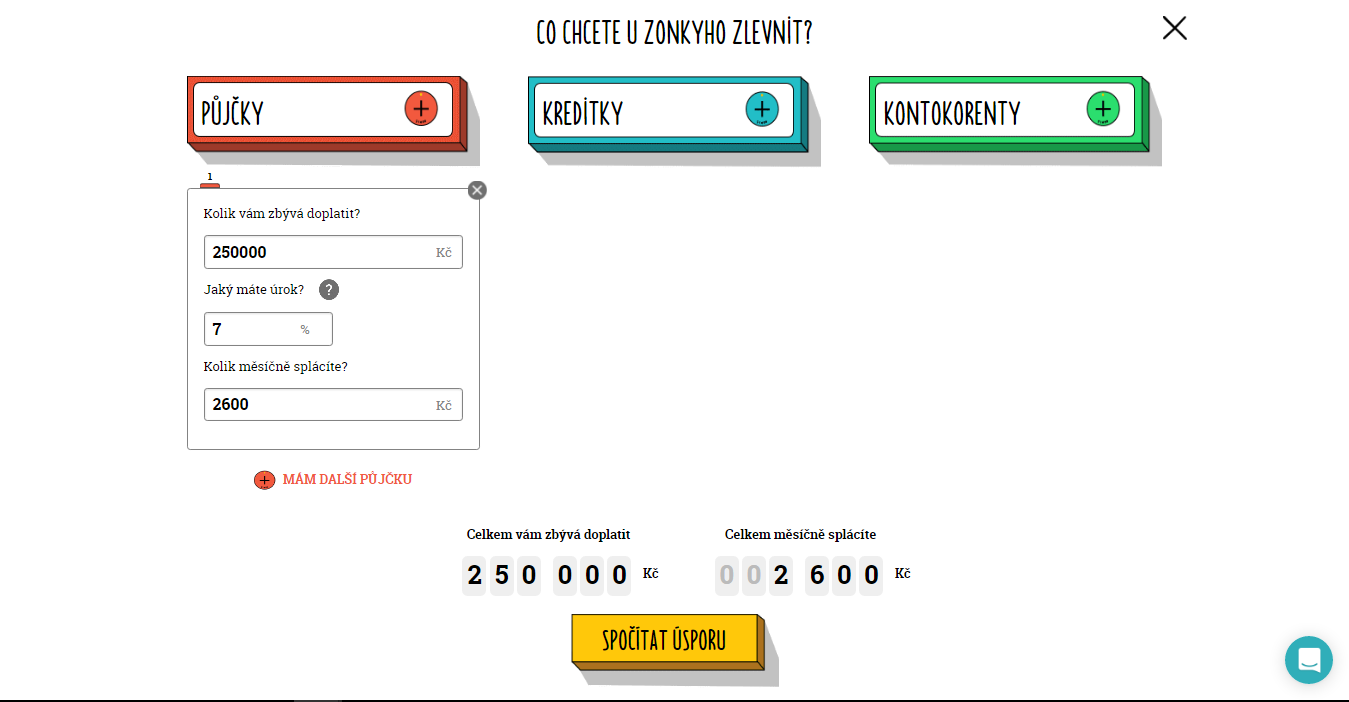
\includegraphics[width=1.0\textwidth]{media/zonky/zlevnovac.png}
    \caption{Zlevňovač na webu Zonky.cz}
    \label{fig:zonky:zlevnovac}
\end{figure}
\begin{figure}[h]
    \centering
    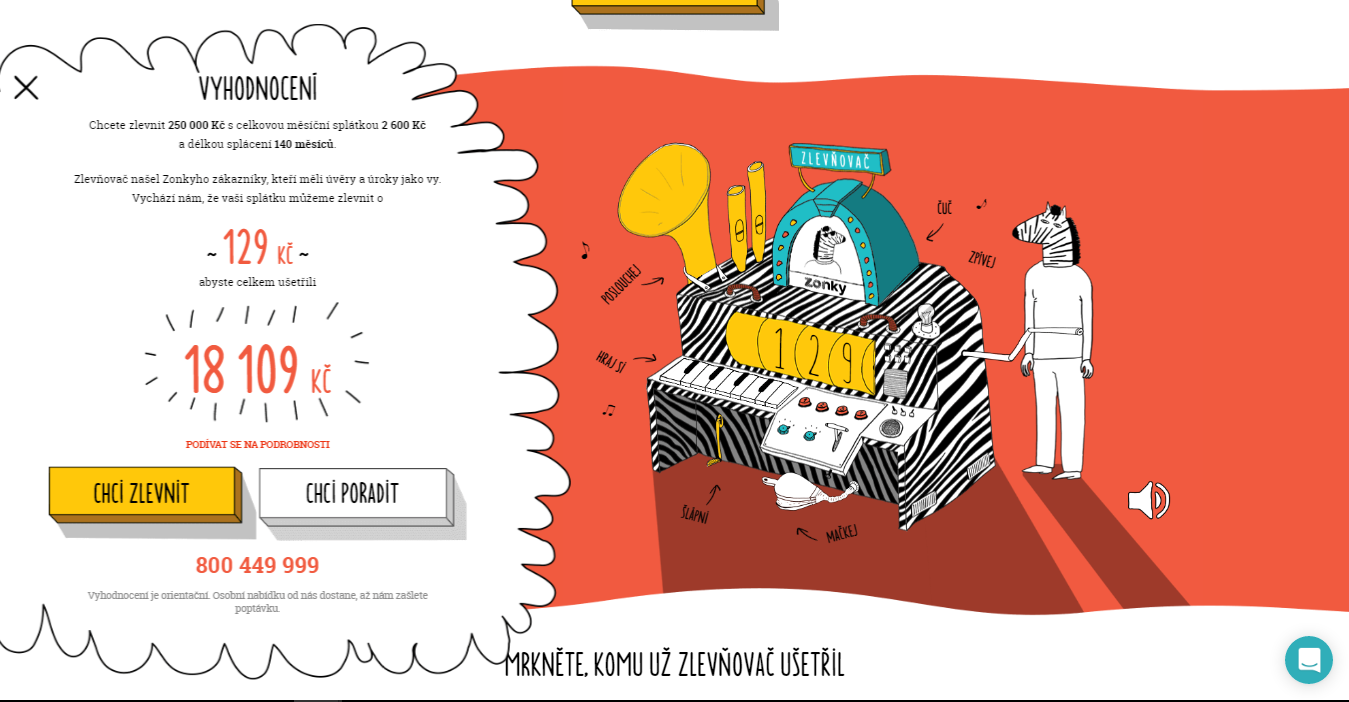
\includegraphics[width=1.0\textwidth]{media/zonky/zlevnovac2.png}
    \caption{Zlevňovač na webu Zonky.cz 2}
    \label{fig:zonky:zlevnovac2}
\end{figure}
\subsubsection*{Pozitiva}
\begin{itemize}
    \item[+] \textbf{Jednoduchost a přehlednost} -- Opět jednoduché uživatelské rozhraní, ve kterém se nachází jen to potřebné.
    \item[+] \textbf{Vyhodnocení} -- Rychlý náhled na to, kolik vlastně ušetřím, podaný pěknou a jasnou formou.
\end{itemize}
\subsubsection*{Negativa}
\begin{itemize}
    \item[-] \textbf{Zvuk}
\end{itemize}


%%%%%%%%%%%%%%%%%%%%%%%%%%%%%%%%%%%%%%%%%%%%%%%%%%%%%%%%%%%%%%%%%%%%%%%%%%%%%%%%%%%%%%%%%%%%%%%%%%%%%%%%%%%%%%%%%%%%%%%%

\newpage
\subsection{Tržiště}
\begin{figure}[h]
    \centering
    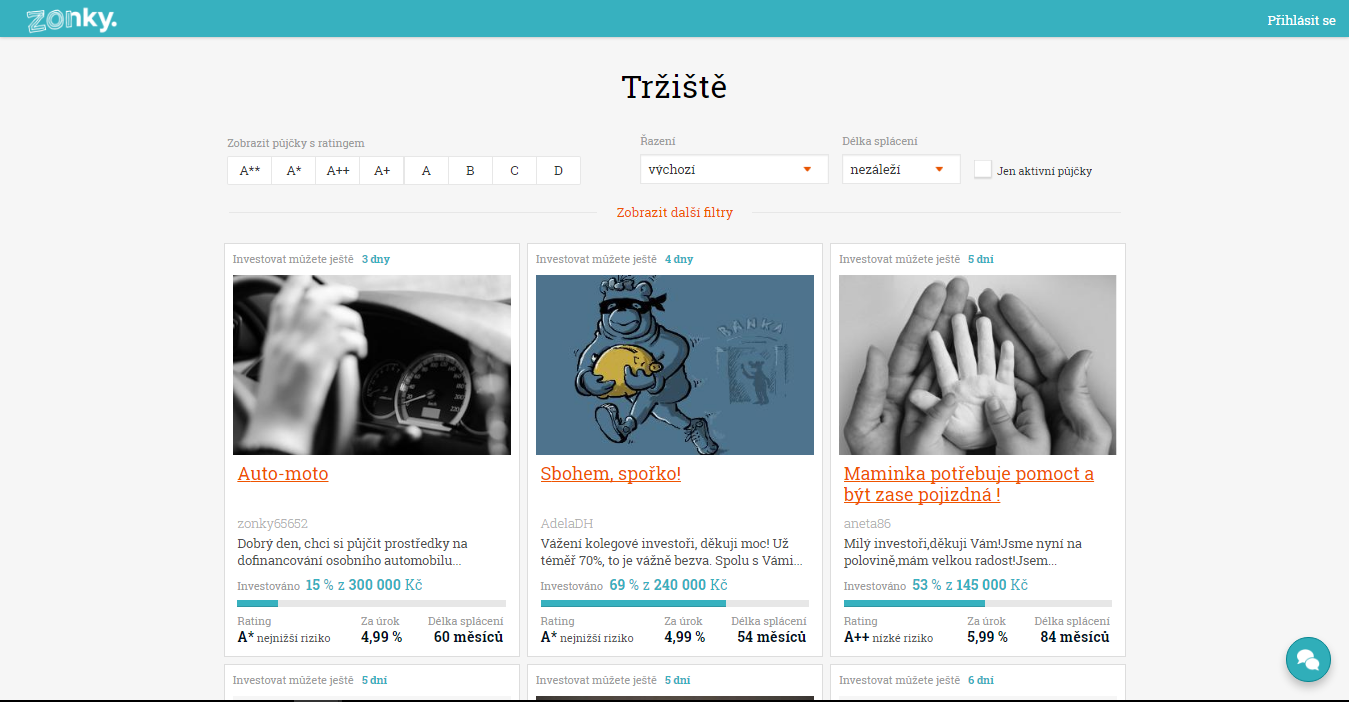
\includegraphics[width=1.0\textwidth]{media/zonky/marketplace.png}
    \caption{Tržiště na webu Zonky.cz}
    \label{fig:zonky:marketplace}
\end{figure}
\subsubsection*{Pozitiva}
\begin{itemize}
    \item[+] \textbf{Informativnost} -- Krátký popis, rating, úrok a doba splácení je vše co uživatel na první pohled potřebuje.
    \item[+] \textbf{Filtry a řazení} -- Uživatel má šanci si rychle zobrazit nabídky, které ho zajímají.
\end{itemize}
\subsubsection*{Negativa}
\begin{itemize}
    \item[-] \textbf{Nevidím}
\end{itemize}


%%%%%%%%%%%%%%%%%%%%%%%%%%%%%%%%%%%%%%%%%%%%%%%%%%%%%%%%%%%%%%%%%%%%%%%%%%%%%%%%%%%%%%%%%%%%%%%%%%%%%%%%%%%%%%%%%%%%%%%%

\newpage
\subsection{Návodné a informativní stránky}
\begin{figure}[h]
    \centering
    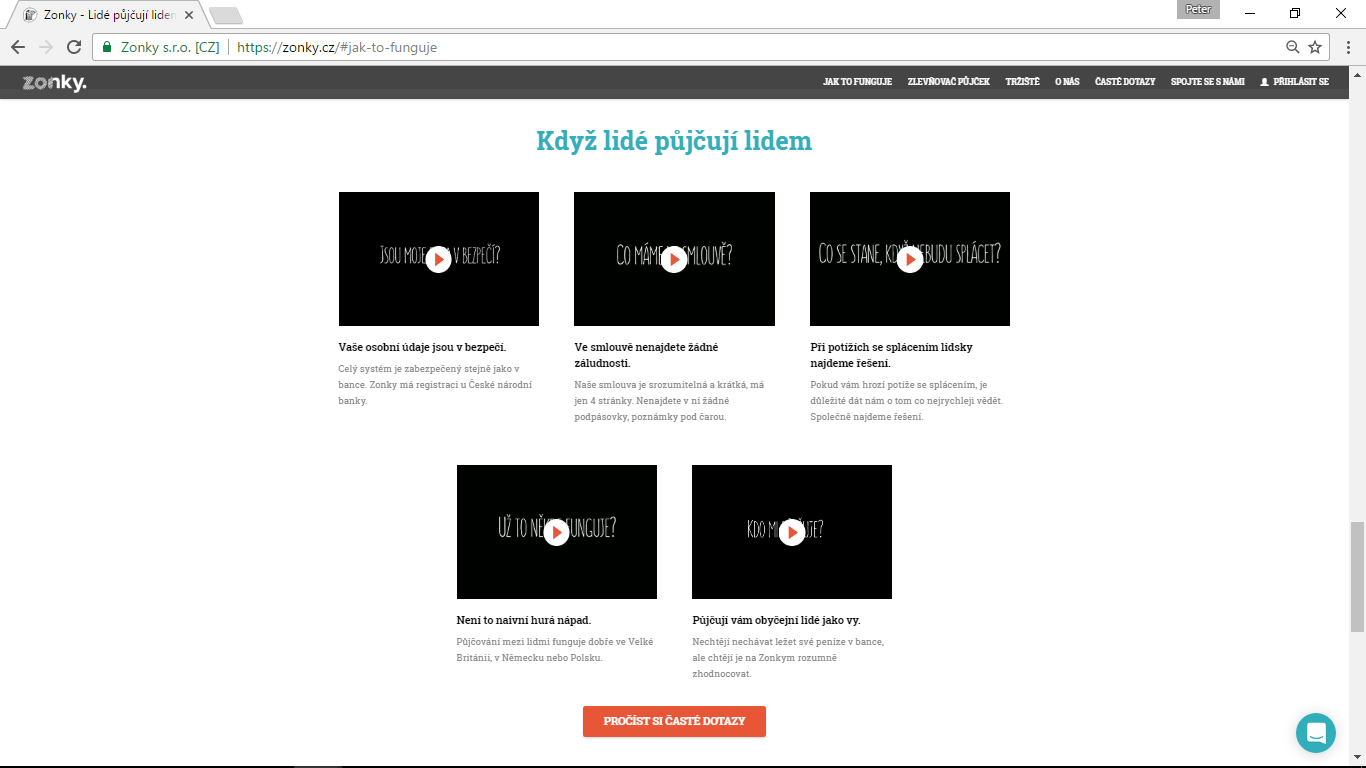
\includegraphics[width=1.0\textwidth]{media/zonky/info.png}
    \caption{Když lidé půjčují lidem -- zonky.cz}
    \label{fig:zonky:info}
\end{figure}
\begin{figure}[h]
    \centering
    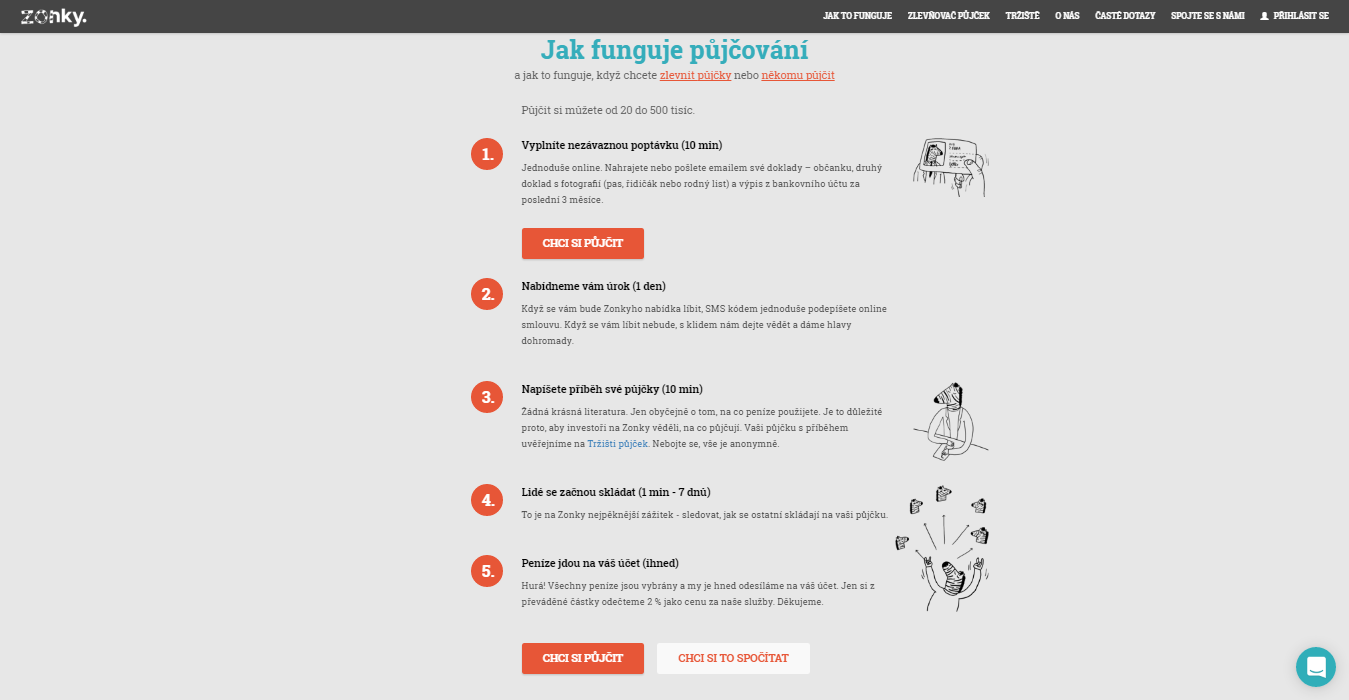
\includegraphics[width=1.0\textwidth]{media/zonky/info2.png}
    \caption{Jak funguje půjčování -- zonky.cz}
    \label{fig:zonky:info2}
\end{figure}
\begin{figure}[h]
    \centering
    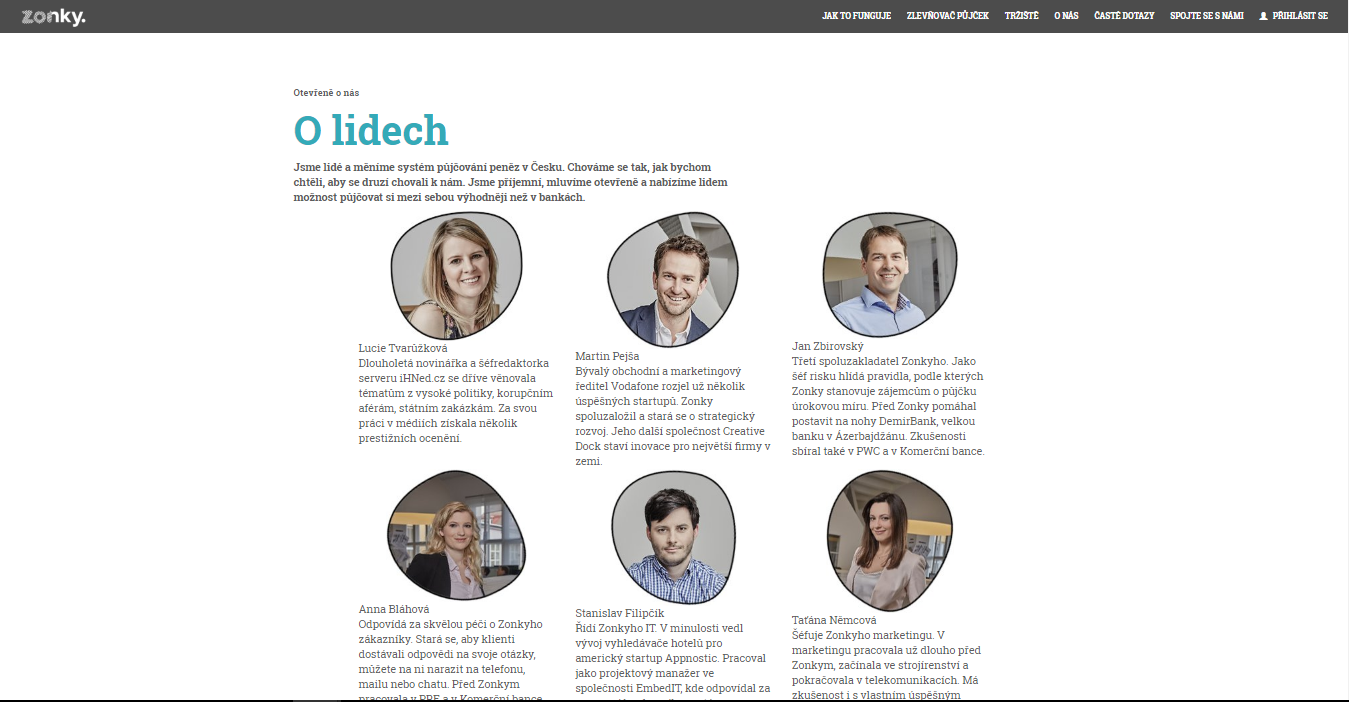
\includegraphics[width=1.0\textwidth]{media/zonky/info3.png}
    \caption{O lidech -- zonky.cz}
    \label{fig:zonky:info3}
\end{figure}
\subsubsection*{Pozitiva}
\begin{itemize}
    \item[+] \textbf{Uživatelská přívětivost} -- Informace podané snadně, jednoduše a přehledně skrz naskrz. Nic není zbytečně rozsáhlé.
\end{itemize}
\subsubsection*{Negativa}
\begin{itemize}
    \item[-] \textbf{Nevidím}
\end{itemize}


%%%%%%%%%%%%%%%%%%%%%%%%%%%%%%%%%%%%%%%%%%%%%%%%%%%%%%%%%%%%%%%%%%%%%%%%%%%%%%%%%%%%%%%%%%%%%%%%%%%%%%%%%%%%%%%%%%%%%%%%

\newpage
\subsection{Shrnutí}
Zonky.cz deklaruje, že chce pomoci lidem, resp. poskytuje možnost pro lidi pomáhat si navzájem. Já chci od své webové aplikace stejnou věc a proto bych se mohl z tohoto řešení něco přiučit.

Pokud chci pomáhat lidem, tak mé uživatelské rozhraní musí být příjemné na používání (to znamená \textbf{jednoduché a přehledné}). Určitě se toho dá dosáhnout i zvolením jiného typu grafiky, ale myšlenka zůstává. Dále si všímám, že v každém zákoutí Zonky se k nám dostává \textbf{dostatečné množství informací} (nejsme zahlcení) a tento princip implementuji také. \textbf{Přítomnost zvuku} je velmi odrazující a určitě tuto chybu nezopakuji v mé aplikaci.